\chapter{Model}\label{chapter:model}
The Dixon and Coles model is one developed for English football that uses full-time scores to predict the probabilities of a future match.  The following will be a deeper look into the football model with modifications made for basketball.

\section{Model Specification}
In order to develop a successful model, there are different features required of a statistical model for basketball games. These features are highlighted by Dixon and Coles for their English football model \citep{dixon_coles}:

\begin{itemize}
	\item The model should consider the different abilities of both teams.
	\item There should be an advantage for the team playing at home.
	\item A team's ability is likely to be based on more recent performances.
	\item A team's ability to score and defend should be summarised separately.
	\item While determining a team's ability, the ability of their opponents should be taken into account.
\end{itemize}

The main assumption of the Dixon and Coles model is that the number of goals scored by the home and away teams in any game are independent Poisson distributions, where the means are determined by each team's attack and defence abilities.  Adjusting this for basketball, in a match between teams $i$ and $j$, let $X_{i,j}$ and $Y_{i,j}$ be the number of points scored by the home and away teams.  Then, 

\begin{equation}
\begin{split}
X_{ij} & \sim \text{Poisson}(\alpha_i\beta_j\gamma),\\
Y_{ij} & \sim \text{Poisson}(\alpha_j\beta_i),
\end{split}
\end{equation}


where $X_{ij}$ and $Y_{ij}$ are independent and $\alpha_i, \beta_i > 0,\ \forall i$.  The team's attack and defence abilities are measured by $\alpha$ and $\beta$ respectively.  The advantage for playing at home is measured by $\gamma$, where $\gamma > 0$.  The probability of a given score between two teams can be calculated by

\begin{equation}\label{eq:base_dc}
\text{Pr}(X_{ij}=x, Y_{ij} = y) = \frac{\lambda^x\exp(-\lambda)}{x!}\frac{\mu^y\exp(-\mu)}{y!}
\end{equation}

where

$$\lambda = \alpha_i\beta_j\gamma,$$
$$\mu = \alpha_j\beta_i.$$

These proabilities can be used to determine the winner of a match, or whether a certain amount of points will be scored.  For example, the probability of a home win in match $k$ is given by:

\begin{equation}
p_k^H = \sum_{x > y} \text{Pr}(X_k = x, Y_k = y)
\end{equation}

A major limitation of this model is that the parameters are static.  The team abilities are considered to be constant throughout time.  This issue will be visited in Section \ref{section:limitation}.


\section{Parameter Estimation}
From model (\ref{eq:base_dc}), with $n$ teams there are $n$ attack and defence abilities along with the home advantage parameter to be estimated.  To prevent the model from being over-parameterized, a constraint of team attack is required:

$$\frac{1}{n}\sum_{i=1}^{n}\alpha_i = 100$$

For the National Basketball Association, there are 30 teams, which gives a total of 61 parameters to be estimated.  To estimate these parameters, a likelihood function is used.  For matches, $k=1,\ldots,N$, with scores $(x_k, y_k)$, this takes the form

\begin{equation}\label{eq:dc_likelhiood}
L_t(\alpha_i, \beta_i,\gamma,i=1,\ldots,n) = \prod_{k=1}^{N} \exp(-\lambda_k)\lambda_{k}^{x_k}\exp(-\mu_k)^{y_k}
\end{equation}

where

$$\lambda_k = \alpha_{i(k)}\beta_{j(k)}\gamma,$$
$$\mu_k = \alpha_{j(k)}\beta_{i(k)},$$

and $i(k)$ and $j(k)$ are the indices of the home and away teams playing in match $k$.  The parameters can be found by maximising (\ref{eq:dc_likelhiood}).  In the NBA, each team plays one another every season.  Table \ref{table:dc_mean} outlines the mean attack and defence parameters for each NBA conference.  As expected, the western conference has a higher average attack and defence rating given their dominance over the eastern conference in previous seasons \citep{western_conference}.

\begin{table}[ht]
\centering
\begin{tabular}{|c|c|c|}
\hline
Conference & Mean $\alpha$ & Mean $\beta$ \\ \hline
Western & 12 & 12 \\ 
Eastern & 123 & 12 \\ \hline
\end{tabular}
\caption{My caption}
\label{table:dc_mean}
\end{table}

\section{Model Limitation and Modification}\label{section:limitation}
The basic limitation of model (\ref{eq:dc_likelhiood}) is that the parameters are static.  All the matches are weighed equally which leads to teams having the same ability parameters over time, when in reality team performance tends to fluctuate.  Especially over the course of multiple seasons where players may change teams.  Teams may go through multiple injuries, winning and losing streaks and multiple other factors.  The current model does not accurately reflect teams' recent form.  In order to compensate for this, Dixon and Coles introduced a modification to the model by adding a factor that will reduce the significance of older matches:

\begin{equation}\label{eq:dc_time}
L_t(\alpha_i, \beta_i,\gamma,i=1,\ldots,n) = \prod_{k=1}^{N} \{\exp(-\lambda_k)\lambda_{k}^{x_k}\exp(-\mu_k)\}^{\phi(t-t_k)}
\end{equation}

In the model, $t$ is the time the estimation was made and $t_k$ is the time match $k$ was played.  Match weighting can be changed by varying $\phi$.  Dixon and Coles chose the model

$$\phi(t) = \exp(-\xi t),$$

where all previous matches are downweighted exponentially based on $\xi > 0$.  When $\xi = 0$, all matches have equal weight, such as model (\ref{eq:dc_likelhiood}).  Larger values of $\xi$ will give more weight to recent matches.  

\begin{figure}[!htb]
	\centering
	\includegraphics[width=0.75\textwidth]{{Figures/xi_accuracy.pdf}}
	\captionof{figure}{Prediction accuracy for different values of $\xi$.}
	\label{fig:xi_accuracy}
\end{figure}

\begin{figure}[!ht]
	\centering
	\begin{subfigure}{0.67\linewidth}
	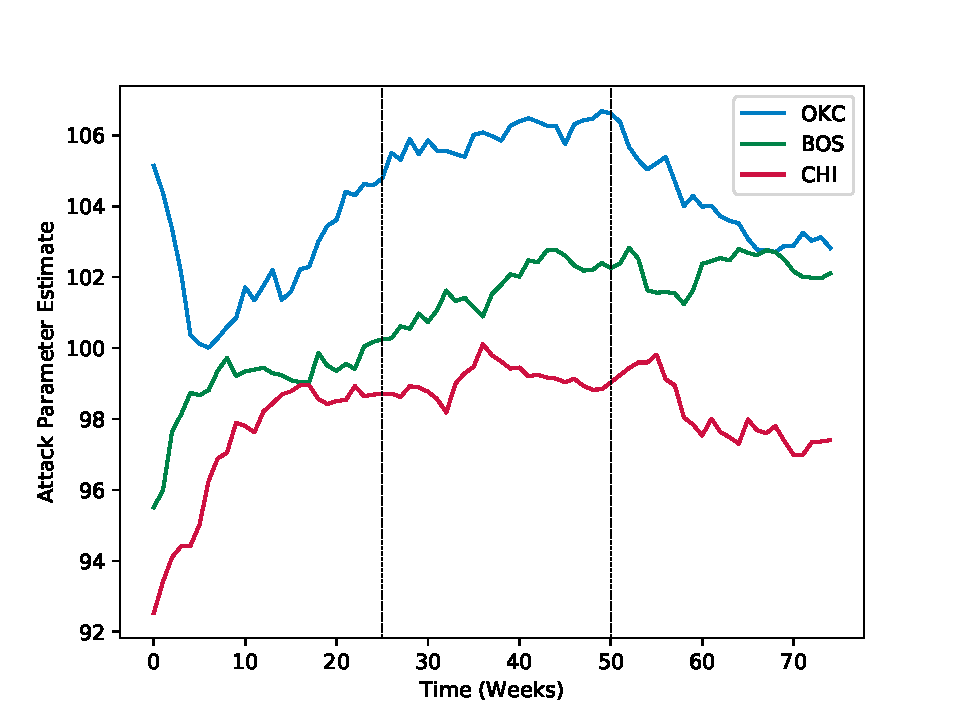
\includegraphics[width=1\textwidth]{{Figures/weeks_attack.pdf}}
	\caption{}	
	\end{subfigure}
	
	\begin{subfigure}{0.67\linewidth}
	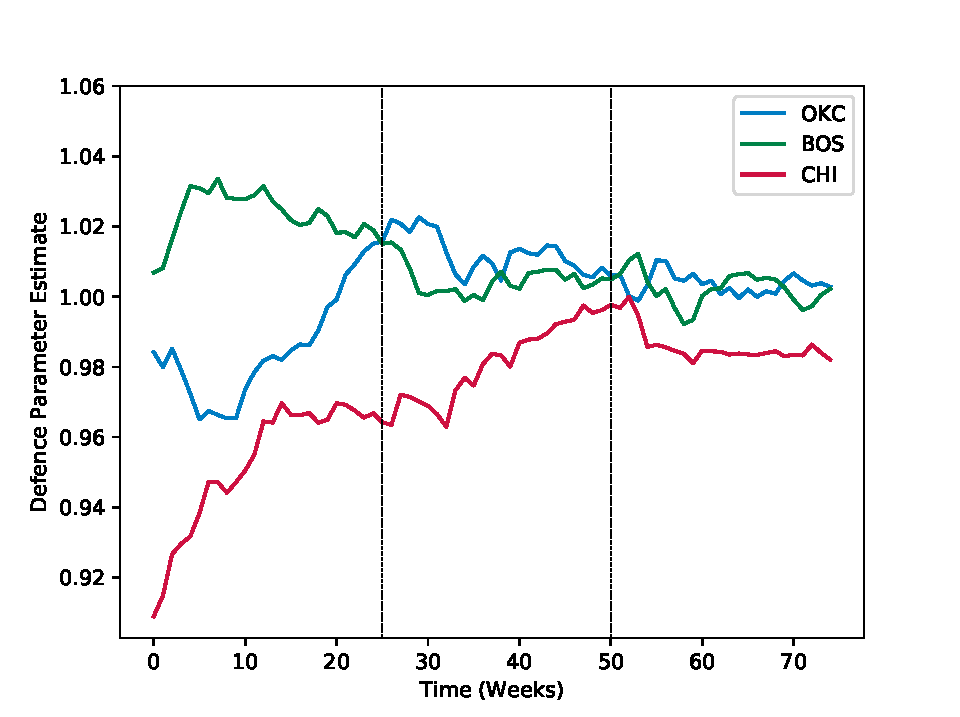
\includegraphics[width=1\textwidth]{{Figures/weeks_defence.pdf}}
	\caption{}
	\end{subfigure}
	
	\begin{subfigure}{0.67\linewidth}
	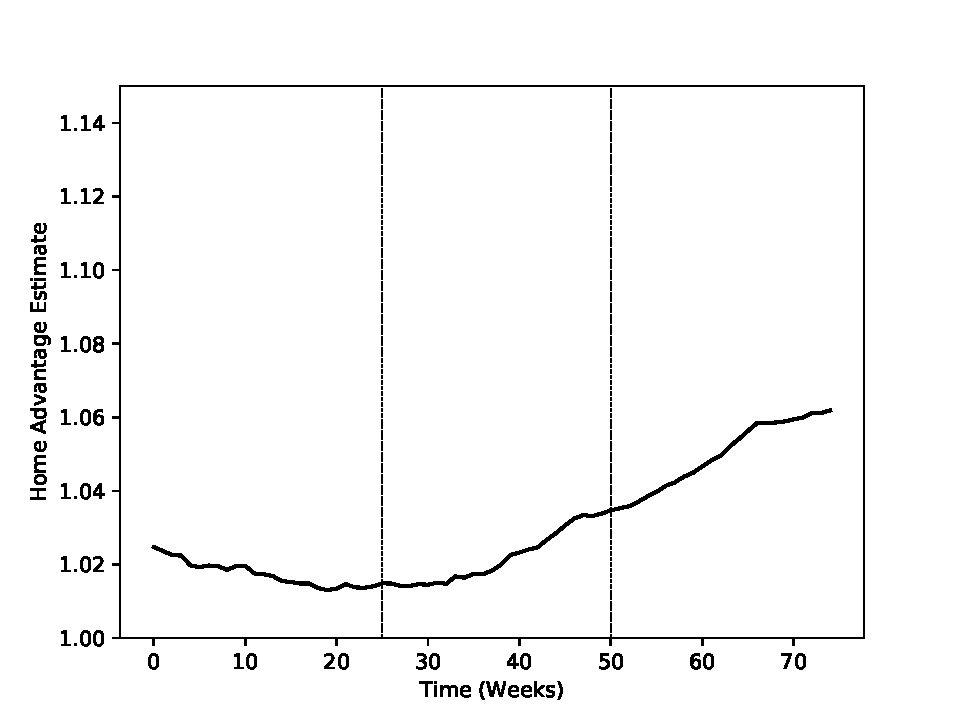
\includegraphics[width=1\textwidth]{{Figures/weeks_home.pdf}}
	\caption{}
	\end{subfigure}
	
	\caption{(A),(B) Attack and defence parameter weekly estimates for the Oklahoma City Thunder, Boston Celtics and Chicago Bulls; (C) Home advantage parameter variation.\label{fig:weeks_dc}}
	
	
\end{figure}



\section{Player Model}
To get a deeper look into a team's performance, it will be useful to analyse the performance of players.  Especially in basketball compared to other sports, where only 5 players are on the court per team at a time.  The beta distribution will be used to evaluate the performance of players, to see what is the percentage of points that they contribute to their overall team.  Just as was done for the team model, the player model will have a match weight in order to accurately rate recent performances.  The parameter will be the same as the team model.  Maximising a player's beta distribution will lead to recent weighting in performance

\begin{equation}
L(\alpha, \beta | X) = \{ \}^{\phi(t-t_k)}
\end{equation}

A team missing their best player due to injury or suspension will.  This leads to the problem of season long injuries and won't account for that, thus a modification needs to be made.

If a team's best players aren't playing, their performance will surely deviate from what is expected of them.  Thus in this situation, we penalize a team's expected points according to the player's beta mean.  Game prediction accuracy improves to 66.97\%.  The team penalty factor needs to be investigated as the prediction accuracy could be improved.  The maximization of the parameter is done in the same method as $\xi$, shown in Figures \ref{omega}.  \textit{Maybe I could find it using maximum likelihood.}

\begin{figure}[!htb]
	\centering
	\includegraphics[width=0.75\textwidth]{{Figures/omega_accuracy.pdf}}
	\captionof{figure}{Prediction accuracy for different values of $\xi$.}
	\label{fig:omega}
\end{figure}

\subsection{Star Player Model}
The NBA has become a star driven league.  Not every team in the league will have a top 10 player which leads to the previous model weighing unfairly towards smaller market teams.  To determine the best players in the league, the beta means where used just like in the previous section.  Instead of teams, players were divided into positions.  The issue that arises now, is to determine which percentile of best players to use for the model.  Using equation .. Figure 3 shows that the 85th percentile is the best fit for accuracy.
